\documentclass[12pt, a4paper]{article}

\usepackage[T1]{fontenc}
\usepackage[utf8]{inputenc}
\usepackage[polish]{babel}
\usepackage[margin=2cm]{geometry}
\usepackage{indentfirst}
\usepackage{amsmath}
\usepackage{enumitem}
\usepackage{graphicx}
\usepackage{textgreek}
\usepackage{float}


\begin{document}
	
	\begin{center}
		\Huge \textbf{Analiza porównawcza wpływu kursu przygotowawczego na wyniki } \\[0.5em]
		\large Sprawozdanie 1 \\[1.5em]
		\Large Martyna Pacyna 287440 \\ Lena Rojecka 287460
	\end{center}
	
	
	\section{Wstęp}
	\section{Testowanie hipotezy dotyczącej średniej}
		W tym zadaniu należało wykorzystać dane przekazane przez prowadzącą, aby przeprowadzić testowanie hipotezy zerowej H0 : $\mu = 1.5$ przeciwko trzem hipotezom alternatywnym. Najpierw wyznaczymy wartość statystyki testowej. To taka funkcja próby, na podstawie której wnioskuje się o odrzuceniu lub nie hipotezy statystycznej. Pierwsze porównanie przeprowadzimy przez wyznaczenie hipotezy testowej. Uzyjemy statystyki testowej Z, ponieważ mamy do czynienia z próbami o rozkładzie normalnym, o dużej wielkości oraz ze znanym odchyleniem standardowym. Wyliczamy go z poniższego wzoru: 
		\begin{equation*}
			Z = \frac{\bar{X} - \mu_0}{\sigma / \sqrt{n}}
		\end{equation*}
		
		Gdzie:
		\begin{itemize}
			\item $\bar{X}$ -- średnia z danych (wyliczona z pakietu numpy dla naszych danych wynosi $\approx 1.45546$),
			\item $\mu_0 = 1.5$ -- wartość z hipotezy zerowej,
			\item $\sigma = 0.2$ -- sztywna wartość z treści zadania,
			\item $n$ -- liczba elementów (w naszym przypadku 1000).
		\end{itemize}
				
		\begin{equation*}
			SE = \frac{\sigma}{\sqrt{n}}
		\end{equation*}
		
		Obliczamy więc, że
		\begin{equation*}
			Z = \frac{\bar{X} - \mu_0}{\sigma / \sqrt{n}} = \frac{1.45546 - 1.5}{0.2/ \sqrt{1000}} \approx \frac{-0.04}{0,00632} \approx -7.04
		\end{equation*}
			\begin{equation*}
			SE = \frac{\sigma}{\sqrt{n}} = \frac{0.2}{\sqrt{1000}} \approx 0.0063
		\end{equation*}
		
		Dla naszych danych $Z \approx -7.04$ co stanowi bardzo rzadki wynik. Obliczyliśmy również błąd standardowy (który jest mianownikiem równania powyżej), z którego wychodzi nam $SE = 0.0063$. Wynik taki wyszedł między innymi dlatego, że nasza średnia z próby $\bar{X} = 1.455$. Jest to wynik mniejszy niż nasz oczekiwany (1.5). Nasza próba jest też bardzo duża, bo stanowi 1000 elementów.  Przy tak gigantycznej próbie, nawet mała różnica od zakładanej średniej staje się znacząca. Taki wynik oznacza, że nasza próba jest bardzo czuła i precyzyjna. \\
		
		Kolejnym krokiem będzie określenie obszaru krytycznego dla każdego przypadku. Jeśli hipoteza zerowa mówi o tym, że coś jest różne, to obszar krytyczny jest dwustronny i zaznaczamy zarówno prawą jak i lewą końcówkę rozkładu. Jeśli hipoteza alternatywna jest sformułowana jako mniejsze lub większe, to zaznaczamy obszar odrzuceń albo z prawej albo z lewej strony.\\
		
		Następnie dla każdej hipotezy alternatywnej obliczymy p-value, czyli wartość p. Jest to prawdopodobieństwo otrzymania wyników równie skrajnych lub jeszcze bardziej skrajnych niż uzyskane w badaniu, przy założeniu że hipoteza zerowa jest prawdziwa. Kolokwialnie mówiąc, jest to "wielkość naszego ogona", ktorego widać na wykresie. Jest TO alternatywny sposób podejmowania decyzjji w testowaniu hipotez.
		Decyzja na podstawie wartości p jest podejmowana przez porównanie wartości p z poziomem istotności $\alpha$. Jeśli p value $\leq \alpha $ odrzucamy hipoteze zerową. Wartość p można interpretować jako najmnijeszy poziom istotności, przy którym moglibysmy odrzucić $H_0$. \\
		
		Zacznijmy od przeanalizowania hipotezy alternatynej [$H_1$: $\mu \neq 1.5$]. Hipoteza alternatywna stwierdza, że badany paramtr rózni się od wartości określonej w hipotezie zerowej. W tym przypadku obszar krytyczny znajduje się w obu ogonach rozkładu statystyki testowej. Odrzucamy $H_0$ jeśli wartość statystyki testowej jest ekstremalnie duża lub ekstremalnie mała. W tym przypadku granica lewostronna była liczona do poziomu $\alpha/2$, a prawostronna $1 - \alpha/2$ za pomocą funcji ppf wbudowanej w pythonie. 
	\
		\begin{figure}[H]
			\centering
			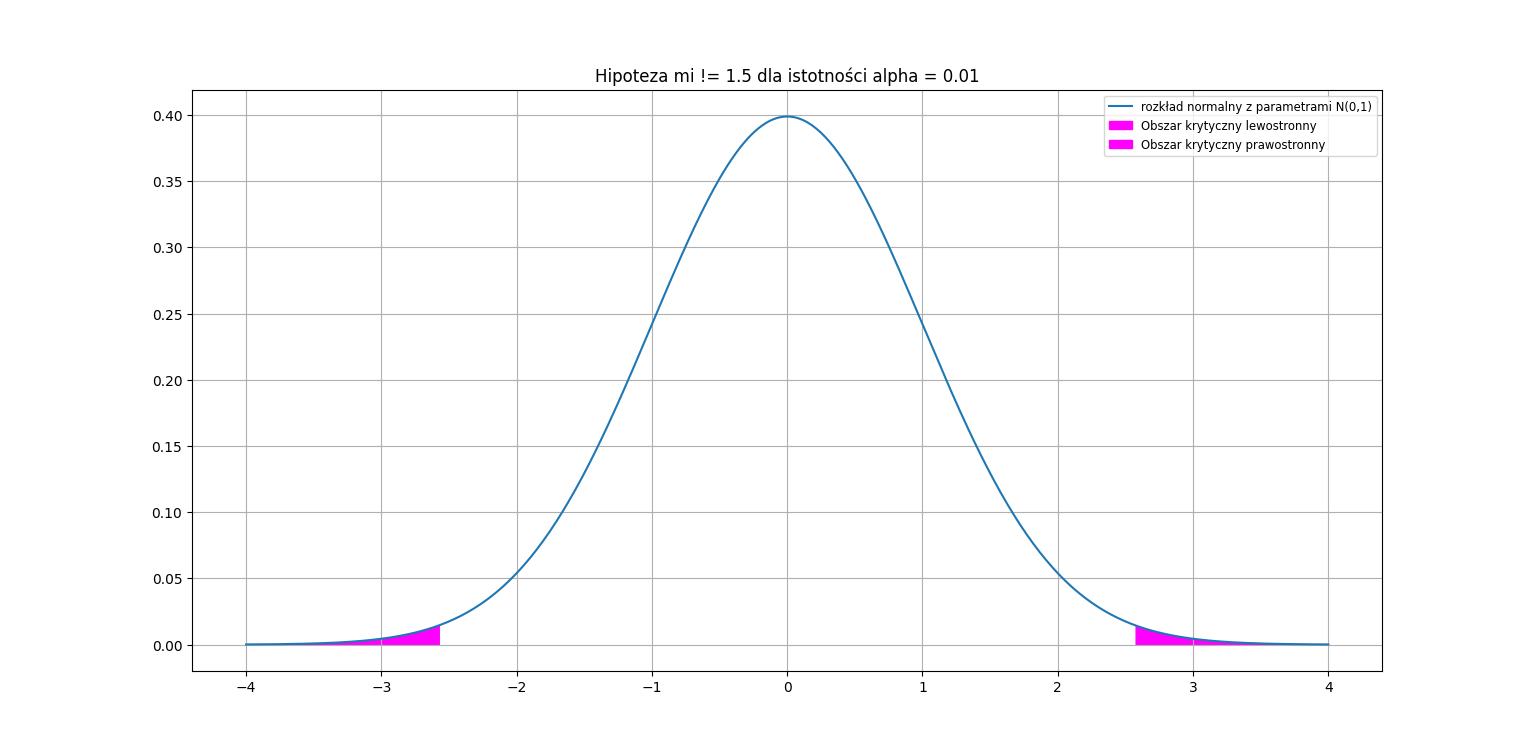
\includegraphics[width=0.8\textwidth]{Figure_1.png} 
		\end{figure}
		\begin{figure}[H]
		\centering
		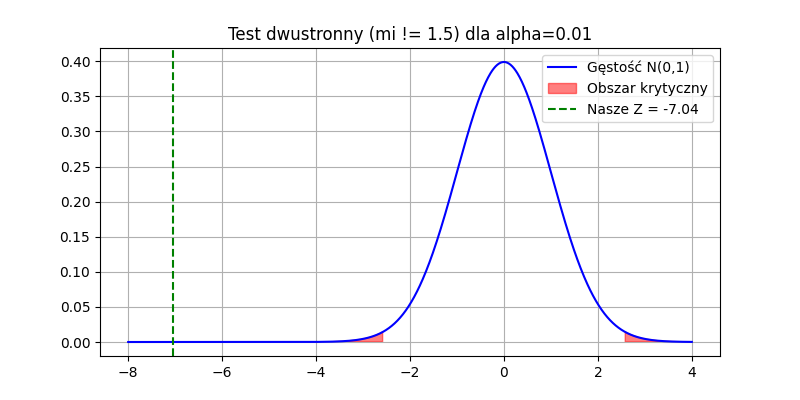
\includegraphics[width=0.8\textwidth]{Figure_2.png} 
		\end{figure}
		\begin{figure}[H]
			\centering
			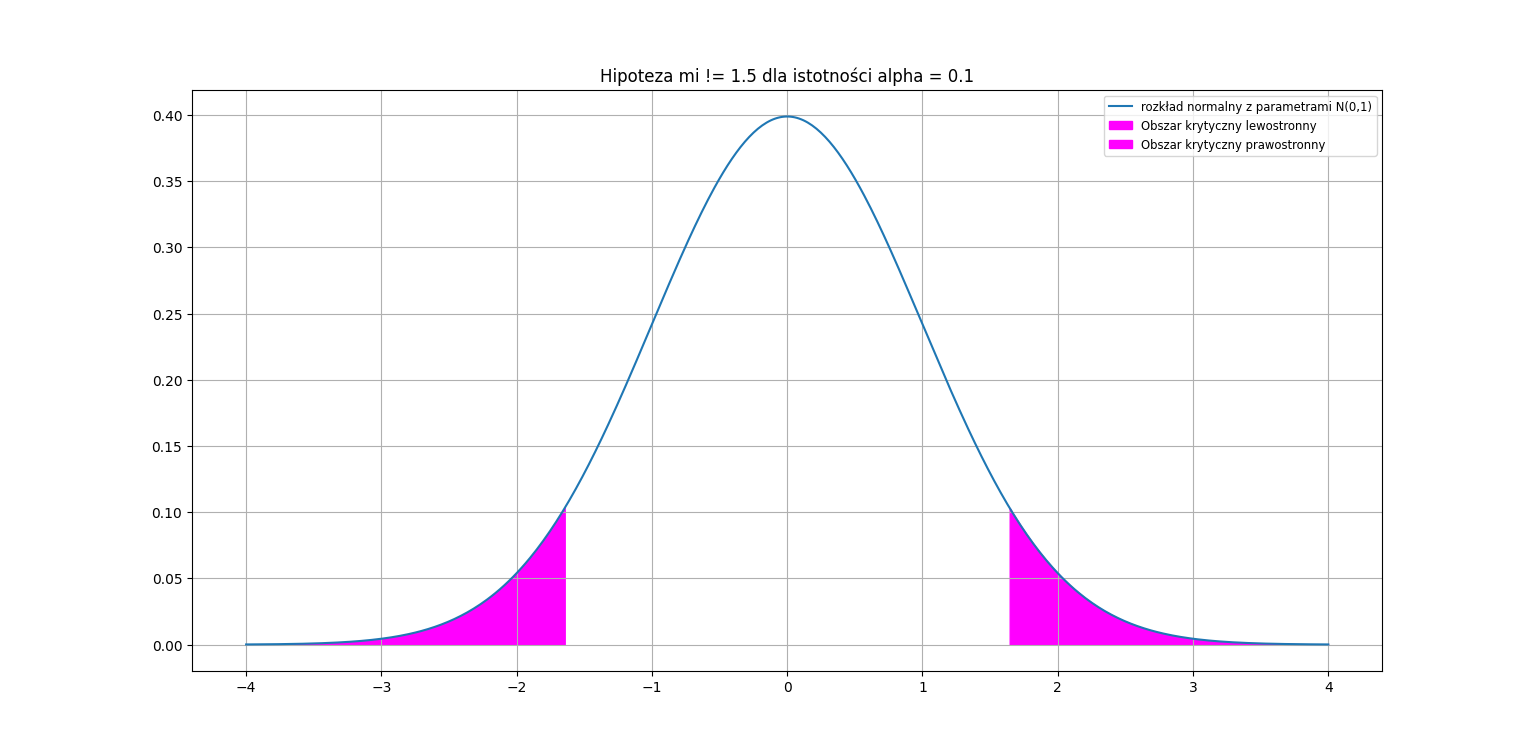
\includegraphics[width=0.8\textwidth]{Figure_3.png} 
		\end{figure}
	\begin{itemize}
		W tym przypadku granice były równe kolejno dla poziomu istotności:
		\item  $\alpha$ = 0.01 \\
		granica lewostronna -2.57, granica prawostronna 2.57
		\item $\alpha$ = 0.05 \\
		granica lewostronna -1.95, granica prawostronna 1.95
		\item $\alpha$ = 0.1 \\
		granica lewostronna -1.64, granica prawostronna 1.64
	\end{itemize}
		Dla testu dwustronnego, $p$-wartość definiujemy jako $$p = P(|Z| \ge |Z_{\text{obs}}|)$$
		Wykorzystując własność wartości bezwzględnej, prawdopodobieństwo to rozbija się na sumę dwóch skrajnych ogonów rozkładu, natomiast z racji idealnej symetrii gęstości rozkładu normalnego, możemy zapisać to równanie za pomocą jednego ogona pomnożonego przez dwa. $F(x)$:$$p = 2 \cdot P(Z \le Z_{\text{obs}}) = 2 \cdot F(Z_{\text{obs}})$$. U nas $Z_{\text{obs}} = -7.04$. Podstawiając wartość statystyki testowej do powyższego wzoru, otrzymujemy wyrażenie za pomocą całki gęstości prawdopodobieństwa rozkładu $N(0,1)$:$$p = 2 \cdot \int_{-\infty}^{-7.04} \frac{1}{\sqrt{2\pi}} e^{-\frac{t^2}{2}} \, dt$$Wartość dystrybuanty dla tego punktu wynosi:
		$$F(-7.04) \approx 9.61 \cdot 10^{-13}$$
		$$p-value = 2 \cdot (9.61 \cdot 10^{-13}) \approx 1.92 \cdot 10^{-12} \approx 0.00000000000192$$ \\
		
		Interpretacja:
		Im większy mamy poziom istotności $\alpha$, tym większe pole ma obszar krytyczny. Wartość p jest bardzo bliska zeru. Oznacza to, że prawie z całą pewnością możemy stwierdzić, że nasza hipoteza alternatywna jest prawdziwa i możemy odrzucić hipotezę zerową.
		
		\newpage
		Kolejną hipotezą alternatywną jest hipoteza	[$H_1$: $\mu > 1.5$]. Hipoteza alterntywna stwierdza, że badany parametr jest większy niż wartość określona w hipotezie zerowej. Obszar krytyczny znajduje się tylko w prawym ogonie rozkładu. Odrzucamy $H_0$, jeśli wartość statystyki testowej jest ekstremalnie duża. 
				\begin{figure}[H]
			\centering
			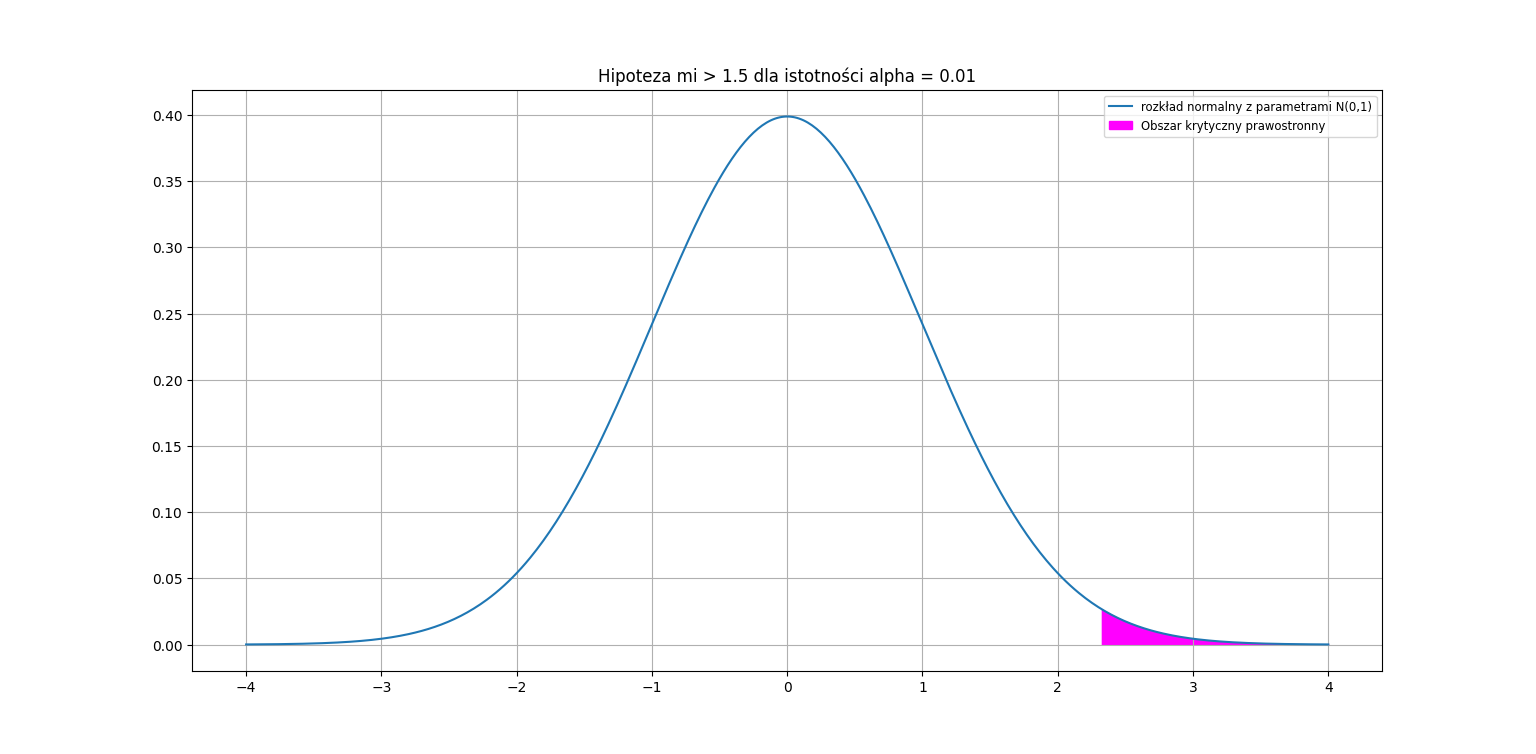
\includegraphics[width=0.8\textwidth]{Figure_4.png} 
		\end{figure}
		\begin{figure}[H]
			\centering
			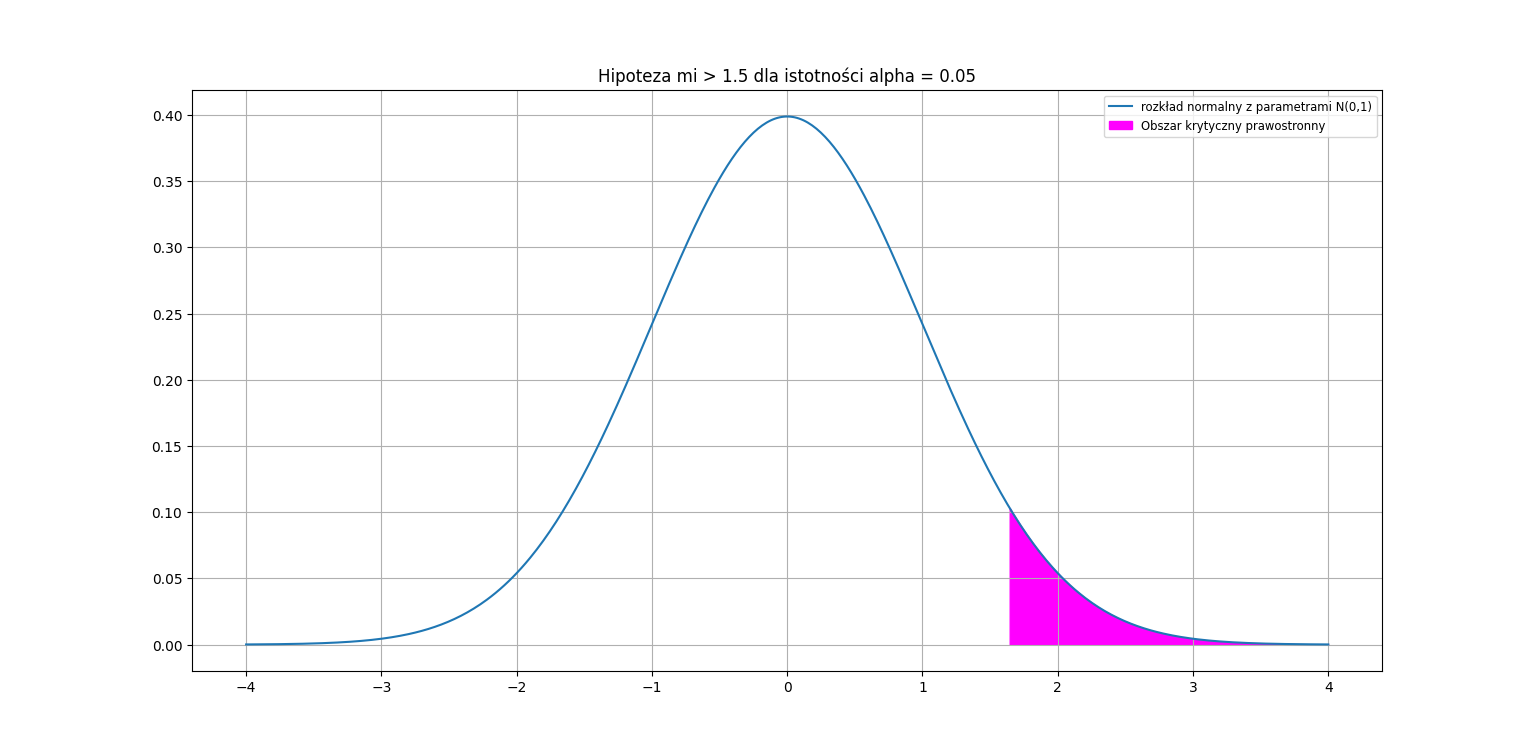
\includegraphics[width=0.8\textwidth]{Figure_5.png} 
		\end{figure}
		\begin{figure}[H]
			\centering
			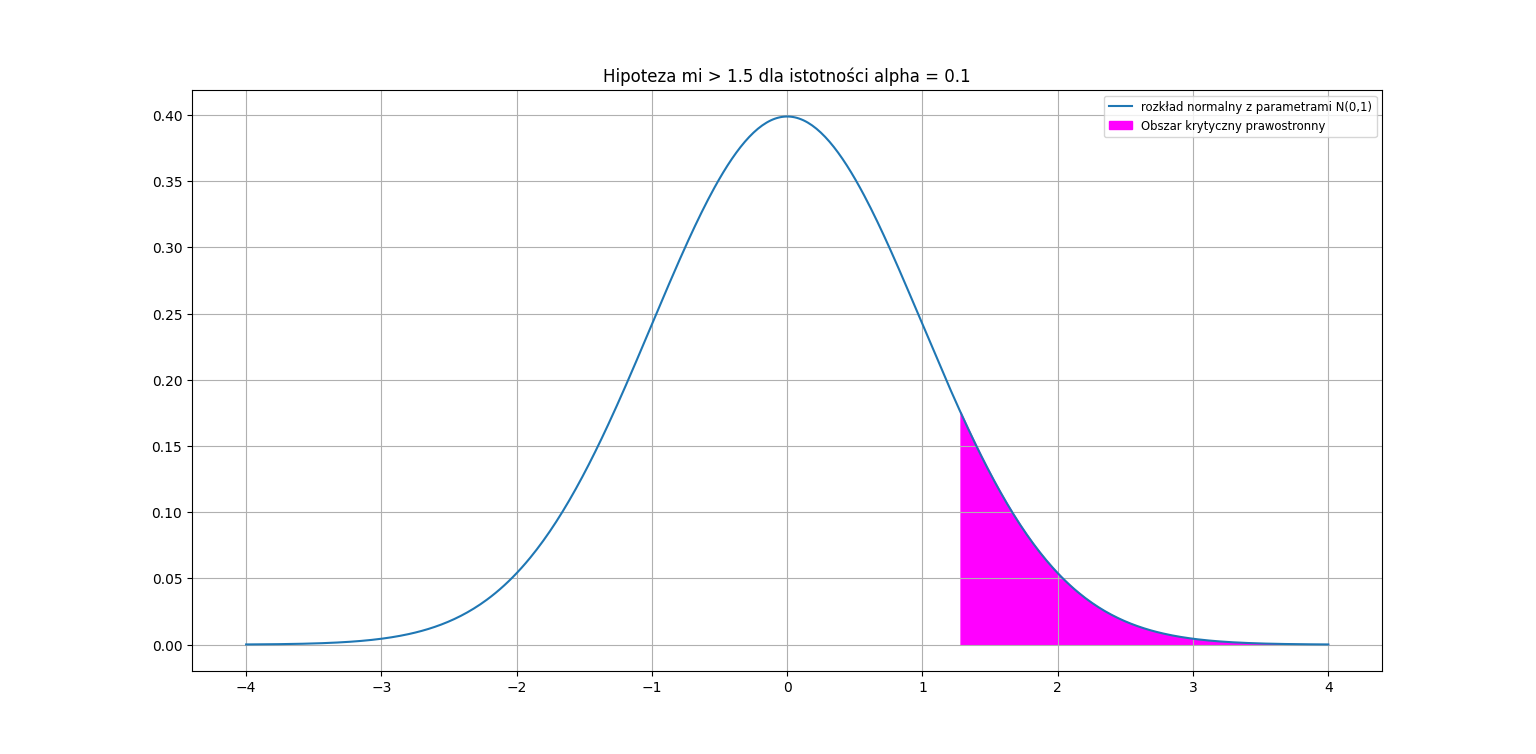
\includegraphics[width=0.8\textwidth]{Figure_6.png} 
		\end{figure}
		
		\begin{itemize}
			W tym przypadku rozpatrujemy jedynie granice prawostronną. Kolejno dla poziomu istotności:
			\item  $\alpha$ = 0.01 \\
			granica prawostronna 2.32
			\item $\alpha$ = 0.05 \\
			granica prawostronna 1.64
			\item $\alpha$ = 0.1 \\
			granica prawostronna 1.28
		\end{itemize}
		
		Dla testu prawostronnego, p-wartość definiujemy jako: 
		$$p = P(Z \ge Z_{\text{obs}})$$Za pomocą dystrybuanty $F(x)$, która domyślnie mierzy pole od lewej strony, prawdopodobieństwo prawego ogona wyrażamy jako: $$p = 1 - F(Z_{\text{obs}})$$
		Podstawiając ujemną wartość statystyki testowej do wzoru, otrzymujemy:$$p = 1 - F(-7.04)$$. Wyrażając to za pomocą całki z funkcji gęstości prawdopodobieństwa rozkładu $N(0,1)$:$$p = \int_{-7.04}^{+\infty} \frac{1}{\sqrt{2\pi}} e^{-\frac{t^2}{2}} \, dt$$Ponieważ punkt $-7.04$ leży ekstremalnie daleko na lewym ogonie, pole na lewo od niego ($F(-7.04)$) jest bliskie zeru. Wobec tego pole na prawo od niego obejmuje niemal cały wykres rozkładu:$$F(-7.04) \approx 9.61 \cdot 10^{-13}$$Odejmując tę wartość od jedności, otrzymujemy ostateczny wynik:$$p-value = 1 - 9.61 \cdot 10^{-13} \approx 0.99999999999904$$ \\
		
		Interpretacja:
		Zwiększanie poziomu istotności alpha zwiększa obszar krytyczny dla obserwacji.Wartość p jest bardzo bliska 1. Oznacza to, że prawie z całą pewnością możemy stwierdzić, że nasze $\mu$ nie będzie większe od 1.5. Tym razem odrzucamy hipotezę alterantywną, a zostajemy przy zerowej.
		
		\newpage
		Ostatnią hipoteza alternatywną, którą bedziemy analizować jest hipoteza [$H_1$: $\mu < 1.5$]. Hipoteza ta stwierdza, że badany parametr jest mniejszy niż wartość okreslona w hipotezie zerowej. Obszar krytyczny znajduje się tylko w lewym ogonie rozkładu. Odrzucamy $H_0$ jeśli wartość statystyki tesotwej jest ekstremalnie mała.
				\begin{figure}[H]
			\centering
			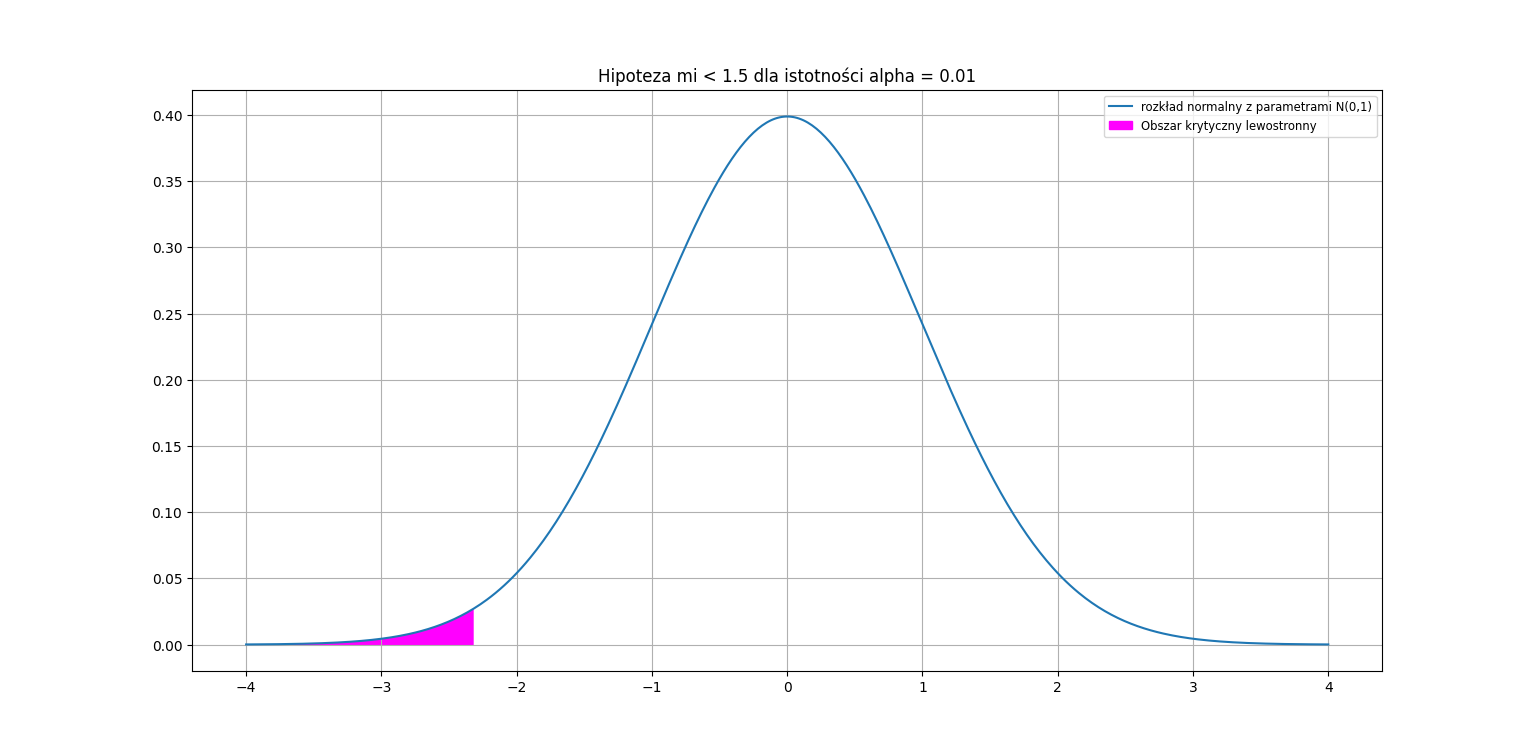
\includegraphics[width=0.8\textwidth]{Figure_7.png} 
		\end{figure}
		\begin{figure}[H]
			\centering
			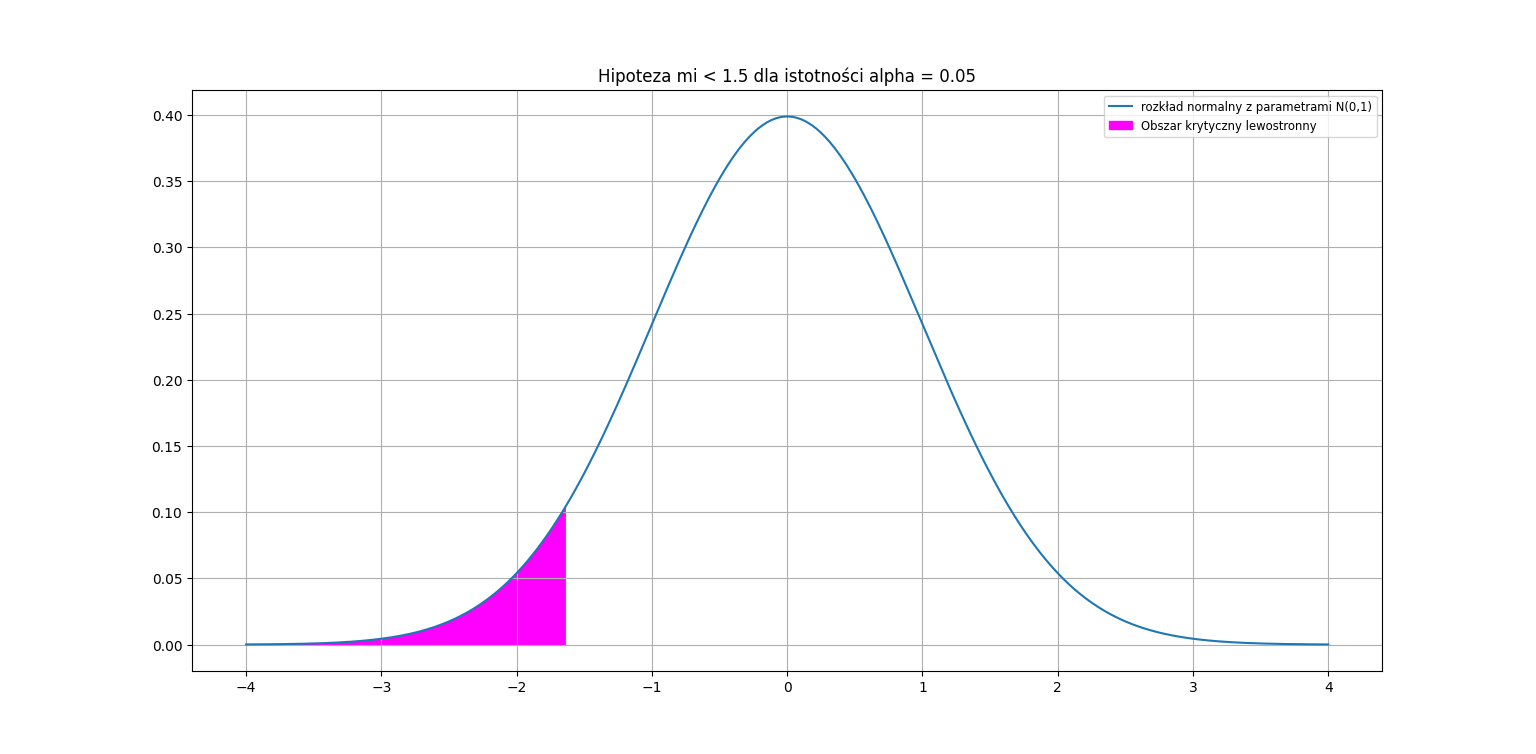
\includegraphics[width=0.8\textwidth]{Figure_8.png} 
		\end{figure}
		\begin{figure}[H]
			\centering
			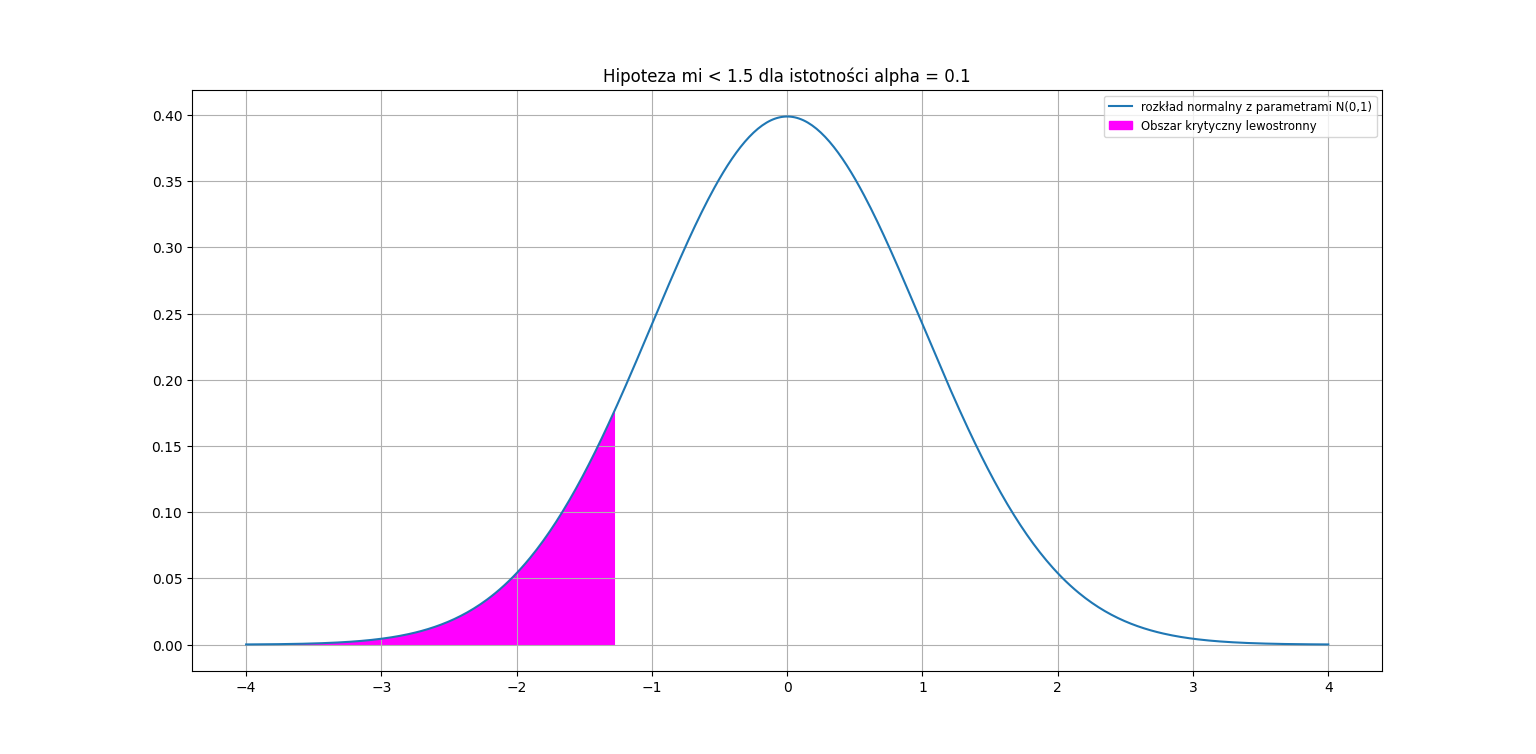
\includegraphics[width=0.8\textwidth]{Figure_9.png} 
		\end{figure}
		
		\begin{itemize}
			W tym przypadku rozpatrujemy jedynie granice lewostronną. Kolejno dla poziomu istotności:
			\item  $\alpha$ = 0.01 \\
			granica lewostronna -2.32
			\item $\alpha$ = 0.05 \\
			granica lewostronna -1.64
			\item $\alpha$ = 0.1 \\
			granica lewostronna -1.28
		\end{itemize}
		
		Dla testu lewostronnego, $p$-wartość definiujemy jako:$$p = P(Z \le Z_{\text{obs}})$$Za pomocą dystrybuanty $F(x)$, która domyślnie mierzy pole pod wykresem od skrajnej lewej strony aż do zadanego punktu, prawdopodobieństwo lewego ogona wyrażamy bezpośrednio jako:$$p\text{-wartość} = F(Z_{\text{obs}})$$Podstawiając ujemną wartość statystyki testowej do wzoru, otrzymujemy:$$p = F(-7.04)$$Wyrażając to za pomocą całki z funkcji gęstości prawdopodobieństwa rozkładu $N(0,1)$:$$p = \int_{-\infty}^{-7.04} \frac{1}{\sqrt{2\pi}} e^{-\frac{t^2}{2}} \, dt$$Ponieważ punkt $-7.04$ leży ekstremalnie daleko na lewym ogonie, pole na lewo od niego (czyli dokładnie nasza dystrybuanta $F(-7.04)$) obejmuje jedynie mikroskopijny skrawek początku wykresu:$$F(-7.04) \approx 9.61 \cdot 10^{-13}$$W tym przypadku nie odejmujemy wartości od jedności, ponieważ interesuje nas wyłącznie obszar lewostronny. Otrzymujemy ostateczny wynik:$$p\text{-value} = 9.61 \cdot 10^{-13} \approx 0.00000000000096$$ \\
		
		Interpretacja:
		Wartość p jest bardzo bliska 0. Oznacza to, że prawie z całą pewnością możemy stwierdzić, że nasze $\mu$ będzie mniejsze od 1.5. Tym razem odrzucamy hipotezę zerową, a zostajemy przy alternatywnej. Możemy też zauważyć, że rozkład ten jest symetryczny do rozkładu prawostronnego, jeśli chodzi o obszary krytyczne. 
\end{document}